% !TeX encoding=utf8
% !TeX spellcheck=en-Us
\hyphenation{mea-sur-ements}
\chapter{Setup}
This chapter presents the experimental setup for electroluminescence measurements. Successful EL measurements consist of injecting charges into the recombination layer, charges recombining and detecting the emitted luminescence. Therefore \autoref{sec:GeneralSetup} explaines the general setup used for EL measurements. \autoref{sec:electricalconnection} explains the Perovskite Cell layout and electrical contacting of the cells, which is used to inject charges into the perovskite layer. The emitted radiation is detected by a camera with the use of additional optics,  explained in \autoref{sec:luminescencedetection}. The chapter concludes with the consideration of noise and measurement errors.

\section{General Setup}\label{sec:GeneralSetup}
The setup is enclosed in a black housing, shielding the inside from outside light and noise (see \autoref{fig:generalsetup}). All parts inside the chamber are painted black to minimize internal reflections and thereby the detection of stray light. A vacuum pump, voltage source, multimeter and operating table with a computer are connected to the setup from the oustide, providing further utility. Inside the enclosure are the probe holder and the camera. The camera is mounted on rails and can be moved in three dimensions, enabling position according to the used optics and samples.
\begin{figure}[h]
	\centering
	\includesvg{Images/ExperimentalSetup/ExperimentalSetupSketch.svg}
	\caption{Schematic of the EL measurement setup. Camera and Probe are positioned inside the setup, and the computer, power supplies and measurement devices are provided from the outside. Two multimeters are used to measure the voltage drop and current sourced.}
	\label{fig:generalsetup}
\end{figure}
\FloatBarrier
\section{Electrical Connection}\label{sec:electricalconnection}
Perovskite Solar Cells (PSCs) are manufactured on 25 mm x 25 mm glass substrates (see \autoref{fig:perolayouttop}). Four cells are deposited on one substrate, each single cell having an active area of 4 mm x 3.5 mm. The cell stack consists of a 0.7 mm thick glass substrate, with a 100 nm thick layer of Indium Tin Oxide (short ITO) deposited ontop. The ITO is structured by laser ablation, isolating the individual cells from each other. Onto the ITO, 10 nm of Spiro-TTB are deposited as a Hole Transport Layer (HTL), followed by 500 nm of methylammonium lead triiodide (short MAPI) as the absorbing material. The top side of the MAPI is contacted with 8 nm of fullerene (short: C$_{60}$) and 23 nm bathocuproine (short: BCP), acting as the Electron Transport Layer (short ETL). In the end of the fabrication process, 100 nm Gold are deposited by thermal vapor deposition on top of the ITO and the C$_{60}$ and BCP. To succesfully contact the PSC a holder with four pins is used. The PSC is positioned face down, with the glass substrate above, onto the holder, positioning the gold pads on all contacts. The holder uses two pins to check proper contacting of the PSC and the other two to source voltage.
\begin{figure}
	\centering
	\includesvg{Images/ExperimentalSetup/Pero_Layout_side}
	\caption{Schematic layout of the perovskite solar cell. Not to scale.}
	\label{fig:perolayouttop}
\end{figure}

The holder is electrically connected to a power supply\footnote{Kukusuki}, in series with a 100 m$\Omega$ resistance, R, and two multimeters\footnote{Keithley 2000 Multimeter} (see \autoref{fig:generalsetup}). One multimeter measures the voltage drop across the PSC. The other multimeter measures the voltage drop across the resistor and the flowing current I is then calculated by Ohm's law:
\begin{equation}
	I = \frac{U}{R}.
\end{equation}
The surface of the holer is structured with rills and conntected to a vacuum pump, fixing the PSC on the holder by a vacuum. This ensures mechanical- and electrical contact stability throughout the measurement.

This setup enables safe contacting of the probes inside the enclosure and thus enables realiable EL measurements.

\section{Luminescence detection}\label{sec:luminescencedetection}
In the setup a CCD camera is used detect the emitted electroluminescence. The camera detects radiation over a wide range of wavelengths, while the perovskite emits luminescence only at a relatively short range of wavelengths. Therefore filters are used to detect only the EL radiation. Optics focus the emitted radiation at a specific distance onto the imaging sensor. This chapter explains the used components and physical processes.
\subsection{Filters}
Between probe and sensor two lowpass filters\footnote{LP714, LP718} are used to filter the wavelengths reaching the detector. In filters absorption or interference are used to either transmit or reflect specific wavelengths. The filters in the setup are two highpassfilters\footnote{LP714, LP718} and chosen accordingly to the luminescence emission spectrum of the PSC (see \autoref{fig:spectrum_perofilter}). This limits the detected wavelengths to above 718 nm, while limiting the detection of straylight with shorter wavelengths. The filters are part of the photoluminescence capability of the setup, where light emitting diodes (LEDs) optically generate charges in the perovskite. To only detect luminescence from the perovskite, both filters block light emitted by the LEDs.

\begin{figure}[h]
	\centering
	\includesvg{Images/ExperimentalSetup/SpectralEL/PL_spectrum_MAPIcell_with_filter_PPT.svg}
	\caption{Emitted luminescence spectrum of the perovskite and transmission function of both filters. }
	\label{fig:spectrum_perofilter}
\end{figure}
\subsection{Optics}
Optics focus the radiation onto a charge coupled sensor (CCD). This setup uses a lens\footnote{Pentax, C2514-M (KP)} with a focus length of 25 mm and an aperature of 1.4, as listed by the manufacturer. The lens is positioned at the minimal object distance of  25 cm away from the PSC. A extender \footnote{Brennweitenverdoppler C - Mount 2-EX / FP-EX2} is mounted directly between camera and lens, with a C-mount, doubling the resultion, however decreasing the intensity reaching the camera.
\\
SKETCH FOR LENS SYSTEM
\\


\subsection{Charge Coupled Detectors}
The radiation is focused onto a charge coupled device (CCD) image sensor\footnote{Sony ICX285-AL} in a camera\footnote{PCO, sensicam qe}. CCD sensors are silicon chips structured into small squares, called wells \cite{SchnellCCD1993}(see \autoref{fig:ccdsensor}). The number of wells correspond to the number of pixel in the taken picture. Radiation generates charges, electrons and holes, and externally applied voltages seperate and trap the charges in the wells. For a specific duration, called exposure time, radiation hits the sensor and charges accumulate in the wells. The amount of generated electrons per incoming photon is called the quantum efficiency (QE), and depends on the sensor material and energy of the photon. The QE for the chosen sensor peaks at 500 nm and decays for larger wavelengths (compare \autoref{fig:pcosensicamqe}). For the wavelengths transmitted by the filter (see \autoref{fig:spectrum_perofilter}), the QE drops to about 10 \%, which limits the sensitivity. After the exposure time a series of voltages is applied to shift the charges from the light sensitive wells to opaque covered wells. Then the charges are extracted row by row and the voltage of each well is measured. An A/D converter convertes the voltage into a digital signal, which is saved and later processed. The camera is connected to a computer by optical fibers and the acquired pictures are processed by the software LabView. The software enables an automatic control of the setup and the acquisition of multiple images in a row.
\begin{figure}
	\centering
	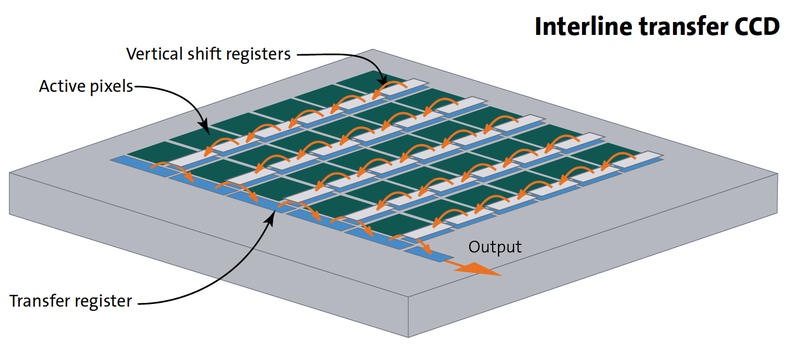
\includegraphics[width=\linewidth]{Images/ExperimentalSetup/ccd-sensor-interline-transfer-en}
	\caption{Schematic represantation of a CCD sensor. Radiation generates charges in the active pixels and is transferred through vertical shift registers to the transfer register. Taken from \cite{StemmerCCD}.}
	\label{fig:ccdsensor}
\end{figure}

This process measures the EL distribution over the PSC surface. However several sources of errors occur, which are discussed in the next section.
%\begin{figure}
%	\centering
%	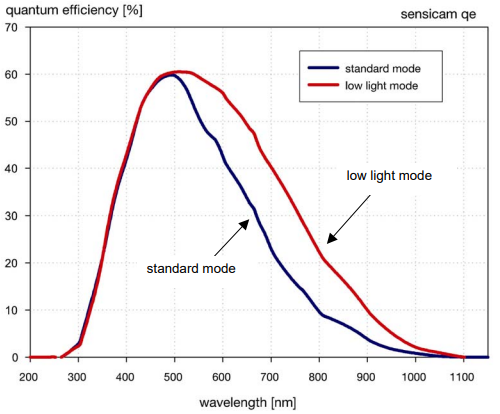
\includegraphics[width=\linewidth]{Images/ExperimentalSetup/PCO_sensicam_QE}
%	\caption{Quantum efficiency of the PCO sensicam qe, given by the manufacturer.}
%	\label{fig:pcosensicamqe}
%\end{figure}
\FloatBarrier
\section{Noise and measurement errors}
Several sources of errors deviate the measured signal from the physical value. Common errors in the camera image acquisition are dark noise, readout noise and hot or cold pixel (see \autoref{table:CCDcamera}). Dark noise refers to the thermal generation of electrons, depending on the temperature and the material's properties. To reduce thermal generation the CCD sensor is cooled to -12 \textdegree C. To further reduce dark noise, images without illumination or applied voltage are taken, and subtracted from the EL image.\\

Readout noise occurs, when the electrons are shifted from well to well. The manufactur specifies the read out noise of 5 electrons. This relates to about two counts, with an analog to digital conversion efficiency of 2 electrons per count \cite{ManualSensicam}. EL images are taken at around 3000 counts, 75 \% of the possible 4096 counts, showing that readout noise can in most cases be neglected. A maximum of two pixels are hot pixels, showing more than 5 electrons,  \\

%ERROR BUGDGET FOR MEASUREMENT\\ 
\begin{table}[h]
	\centering
	\caption{Overview of the characteristic data for the sensicam qe. Specified by the manufacturer \cite{ManualSensicam}.}
	\label{table:CCDcamera}
	%\vspace{0.5cm}
	\begin{tabular}{l c}
		\hline
		& \textbf{Sensicam qe} \\ \hline
		Number of pixels & 1376 x 1040 \\
		Pixel Size & 6.45 $\mu$m x 6.45 $\mu$m \\
		CCD Temperature & -12 \textdegree C \\
		Full Well Capacity & 18000 e$^-$ \\
		Readout Noise & 4...5 e$^-$ \\
		A/D Conversion Factor & 2 e$^-$/count \\
		Average Dark Charge & < 0.1 e$^-$/pixel sec \\
		Warm Pixels > 5e$^-$ & 0...2 \\
		Delay sensicam LONG EXPOSURE & 1 ms ... 1000 s \\ \hline
	\end{tabular}
\end{table}